\documentclass[11pt,a4paper,oneside]{article}
\usepackage[a4paper,top=2cm,bottom=2.5cm,left=2.5cm,right=2cm]{geometry}
\usepackage[T1]{fontenc}
\usepackage[utf8]{inputenc}
\usepackage[english]{babel}
%\usepackage{frontespizio}
\usepackage{graphicx}
\usepackage{subfig}
\usepackage[english]{varioref}
\usepackage{csquotes}

\begin{document}

%opzione per doppio interlinea
\baselineskip 22pt


%Indice%
\tableofcontents\thispagestyle{empty}\clearpage

\section{Introduction}
\pagenumbering{arabic}
\baselineskip 12pt

This project includes various analyses and classifications related to mammogram images. \\
You can refer to these \textit{ipynb} files to verify the code we worked on:\\ \\
Task 2.1:
\begin{itemize}
\item \textit{Scratch\_CNN\_2.1.1 (no data aug)} is the first implementation
\item \textit{Scratch\_CNN\_2.1.2 (data aug)} is the implementation with data augmentation
\item \textit{Scratch\_CNN\_2.1.3 (holdout val)} is the final validation of the best model and the training used for saving the model "scratch\_cnn\_1"
\end{itemize}
Task 2.2:
\begin{itemize}
\item \textit{Scratch\_CNN\_2.2.1 (data aug)} is the implementation with data augmentation
\item \textit{Scratch\_CNN\_2.2.2 (holdout val)} is the final validation of the best model and the training used for saving the model "scratch\_cnn\_2"
\end{itemize}
Task 3.1:
\begin{itemize}
\item 
\end{itemize}
Task 3.2:
\begin{itemize}
\item 
\end{itemize}
Task 4:
\begin{itemize}
\item \textit{Baseline\_CNN\_1} is the implementation of a classification between mass and calcification, using also the baseline patches
\end{itemize}
Task 5:
\begin{itemize}
\item \textit{Ensemble\_1} is the implementation of the ensemble learning for the first classification
\item \textit{Ensemble\_2} is the implementation of the ensemble learning for the second classification
\end{itemize}


\section{The dataset}
The data on which we work are based on the \textbf{CBIS-DDSM} (Curated Breast Imaging Subset of Digital Database for Screening Mammography): it is a set of scanned film mammography studies, adapted to carry out an \textbf{abnormality diagnosis classification}. Following the detailed description attached to each original image, they can be divided into four classes that distinguish whether the represented abnormality patch is a mass or a calcification, and again whether it is benign or malignant. \\
From each original image, the abnormality patch was extracted, and in addition a patch of healthy tissue, adjacent to each abnormality patch, was also extracted. Both abnormality patches and baseline patches have been resized to shape $(150x150)$ and have been added to the final images tensor, that counts 5352 elements (2676 abnormality patches and 2676 baseline patches).
Finally class labels have been assigned to the patches according to the following mapping:
\begin{itemize}
\item 0: Baseline patch
\item 1: Mass, benign
\item 2: Mass, malignant
\item 3: Calcification, benign
\item 4: Calcification, malignant
\end{itemize}

\section{Task 1: Related works}
\begin{itemize}
\item [1] Transfer Learning and Fine Tuning in Breast Mammogram Abnormalities Classification on CBIS-DDSM Database (Lenin G.Falconi, Maria Perez, Wilbert G.Aguilar, Aura Conci) 2020
\item [2] Deep Learning for Breast Cancer Diagnosis from Mammograms - A Comparative Study (Lazaros Tsochatzidis, Lena Costaridou, Ioannis Pratikakis) 2019
\item [3] Automatic Mass Detection in Mammograms Using Deep Convolutional Neural Networks (Richa Agarwal, Oliver Diaz, Xavier Lladó, Moi Hoon Yap, Robert Martí) 2019
\item [4] Multi-View Feature Fusion Based Four Views Model for Mammogram Classification Using Convolutional Neural Network (Hasan Nasir Khan, Ahmad Raza Shahid, Basit Raza,
Amir Hanif Dar, Hani Alquhayz) 2019
\end{itemize}

The first paper, working on our same dataset, deals with the classification of abnormalities using ImageNet pretrained convolutional networks, with the technique of transfer learning (TL) but also fine tuning (FT). The authors specify that the main obstacle for this kind of problem is that there are not yet mammogram public datasets that are quite extensive and "deep", and consequently if we have few data it is difficult to avoid overfitting. The proposed approach, both with TL and FT, consists in replacing the last fully connecting layer related to the original ImageNet classification task with a set of layer: Global Average Pooling 2D, Full Connecting, Dropout, and Classification Layer. They focused on ìly on the masses images, that are initially pre-processed to enhance contrast, then normalized between 0 and 255, and finally rearranged by data augmentation. The dataset was increased to a total of 60.000 images, where 80\% are used for training, 10\% for validation, and 10\% for testing. Looking at the results of TL, they obtained the best AUC with the Resnet-50, that although overfitted. On the other hand, both VGG16 and VGG19 did not presented overfitting but their classification performance were lower. Regarding to FT instead, the best resultes were obtained by VGG16, unfreezed once from the 8th layer and once from the 10th layer, and by VGG19, unfreezed from the 17th layer.

In the second paper, the authors worked on both the CBIS-DDSM dataset and another dataset, the DDSM-400, again to perform a classification of masses between benign and malignant. The initial approach presented is based on training networks from scratch (starting from the Glorot initialization), while later an approach using networks pretrained on the ImageNet datased is presented. They used data augmentation, in particular rotation and flipping transformations, performed online. 
The best results were achieved with CNNs trained under the fine tuning scenario: maximum performance is found with Resnet-50 and Resnet-101. Regarding the networks from scratch, the authors explain that the lowest results are due to the limited number of samples in the analyzed dataset: they say that in these cases \enquote{effective training of larger and complex networks cannot be achieved}.

In the third paper, a patch detector was initially developed, again from the CBIS-DDSM dataset, giving as input to the tested networks patches of abnormal and baseline tissue extracted from mammograms. The authors have used the pretrained networks VGG16, Resnet-50, and InceptionV3, with a transfer learning approach. Since the available images were in black and white, they were replicated on three channels to be compatible with the ImageNet pretrained networks. In addition, the data were augmented on-the-fly using horizontal flipping, rotation, and rescaling. The results of training the CNN on CBIS-DDSM demonstrated that the feature domain of the CNN can be well adapted from natural images to classify masses in mammograms. The best performance were obtained with the InceptionV3.

The last paper were studied mostly for the preprocessing of the data. The experiments in this paper are carried on the CBIS-DDMS and mini-MIAS public databases. First of all, the authors performed some pre-processing steps like rescaling, bilateral filtering, contrast enhancement, on the data for achieving better performance. Then they applied data augmentation transformations to minimize the effect of overfitting, getting a dataset seven times bigger than the original one. Starting from some CNN architectures for training and fine tuning, the authors made adaptations for classification of mammograms on different levels (i.e. normal/abnormal, mass/calcification, and malignant/benign). 


\clearpage

\section{Data Preprocessing}
In this section we describe the main preprocessing applied to the data before the training of the models. Starting from the numpy arrays of the dataset images we were given, first of all we deleted all the samples associated with the \textit{baseline patch} label. Since this labeled images were placed in the even positions of the dataset, we just selected all the odd-index samples and discard the others. This is done both for the training data and the test data. \\
Then we aggregated the labels according to the classification that we needed to do: in the $Task\ 2.1$ and $3.1$ the classes \textit{mass benign} and  \textit{mass malignant} were aggregated in a unique class \textit{mass}, and so for the \textit{calcification} classes. On the other hand, in the $Task\ 2.2$ and $3.2$ we aggregated  \textit{mass benign} and  \textit{cacification benign} in the \textit{benign} class, and the other labels in the \textit{malignant} class.

\begin{figure}[h]
\centering
	\subfloat[][$Task\ 2.1$: 0 for \textit{mass}, 1 for \textit{calcification} \label{fig:label_mass_calc}]
		{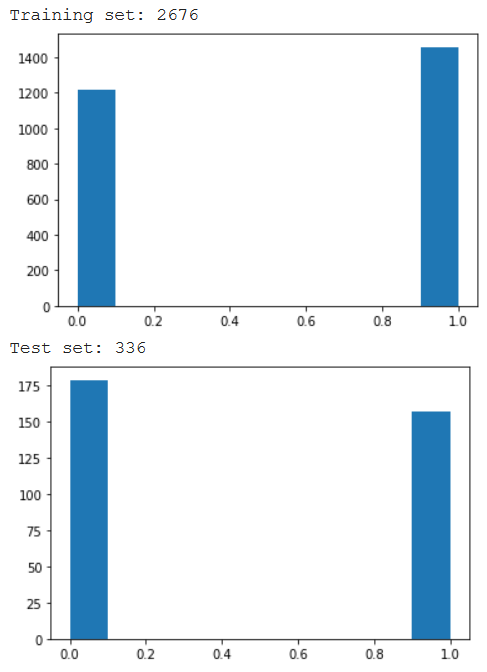
\includegraphics[width=.3\textwidth]{images/label_mass_calc}} \quad
	\subfloat[][$Task\ 2.2$: 0 for \textit{benign}, 1 for \textit{malignant} \label{fig:label_benign_malign}]
		{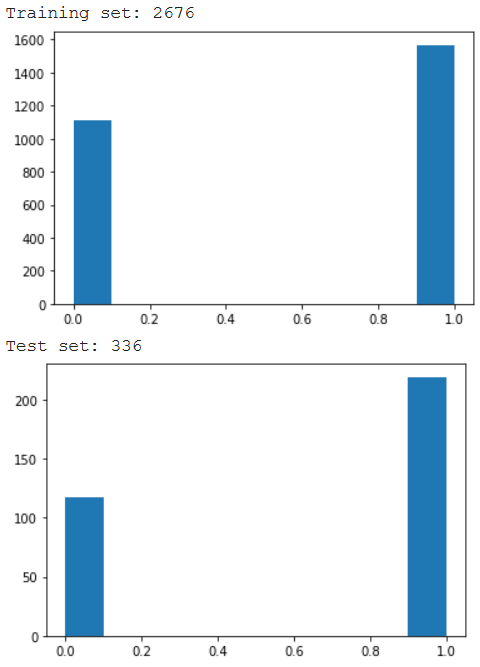
\includegraphics[width=.3\textwidth]{images/label_benign_malign}} \\
\caption{Label distribution}
\label{fig:label distribution}
\end{figure}

For the first case, we can see from the figure that the labels are pretty much equally distributed. Instead, in the second case the dataset is a little more unbalanced towards the \textit{benign} class. \\
Finally, we reshaped all the training images tensors in a single \textit{numpy} array, that has been then normalized. The same has been done for the test images. 
%With regards to the labels, they has been categorizated so that is possible to use the categorical loss function in the model.


\section{Task 2: From Scratch CNN}
We developed different models of neural networks to work with the given dataset from scratch and we did different tests to find the better hyperparameters to build the final model. This section is divided in two parts: i ìn the first one we show how we built a model for classifying the dataset images between \textit{mass} abnormality and \textit{calfication} abnormality, while in the second part we describe the model built to classify between \textit{benign} and \textit{malignant} abnormalities.

\subsection{Task 2.1: Mass-Calcification discriminator}
We first tried to build a simple CNN, with some convolutional and max-pooling layers, and two final dense layers. We trained and tested the model several times, changing the hyperparameters to find a good model for our problem. The final architecture that has been used for the most relevant tests is shown in figure~\ref{fig:scratch_model}. It is made of five convolutional layers, with an increasing number of kernels. Each layer is followed by a max-pooling of $2x2$, except for the last one so that the input of the dense layer is not too reduced. The activation function used in the layers is \textit{ReLu}.

\begin{figure}[h]
\centering
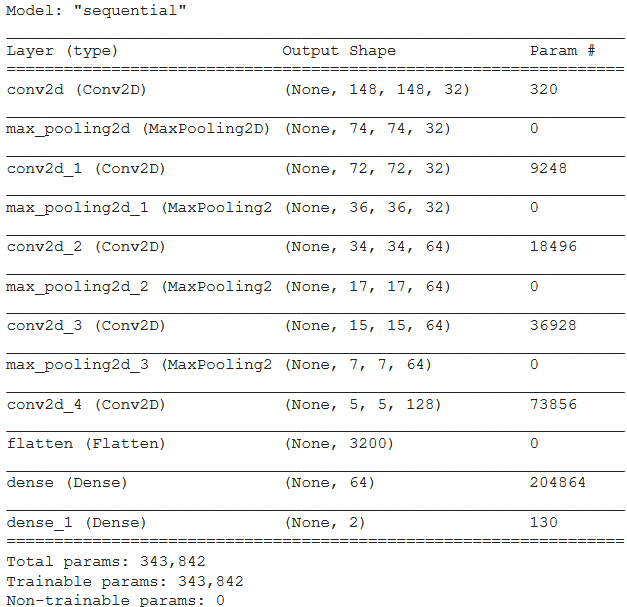
\includegraphics[width=.5\textwidth]{images/scratch_model}
\caption{Architecture of the CNN from scratch ($Task\ 2.1$)}
\label{fig:scratch_model}
\end{figure}

After asserting the architecture, the model has been trained with different numbers of \textit{hidden units} for the first fully connected layer, but also for different \textit{batch sizes}, different \textit{output functions} and different \textit{optimizers}. 
In all the tests, the conclusion has been that the network was over-training, and this is the reason for which we have developed a second model, adding a data augmentation preprocessing. 
In the figure~\ref{fig:scratch_accuracy}, we present the results in term of accuracy and loss, but also the consufion matrix (fig.~\ref{fig:scratch_matrix}), related to a test of the model with $64$ hidden units, a batch size of $25$, and the \textit{softmax} function for the output layer. 
The used optimizer was \textit{Adam}, with the deafult learning rate of $0.001$. As we said before, the gap between the training and validation graphs shows that the model is over-training: even if the predictions on the test set are accurate, we cannot rely on this network as it is.

\begin{center}
\begin{tabular}{|l|ccc|}
\hline
 & Training set & Validation set & Test set \\
\hline
accuracy & 0.9982 & 0.8134 & 0.8244 \\
loss & 0.0123 & 1.1618 & 1.5748 \\
\hline
\end{tabular}
\end{center}

\begin{figure}[h]
\centering
	\begin{minipage}[c]{.35\textwidth}
		\centering\setlength{\captionmargin}{0pt}%
		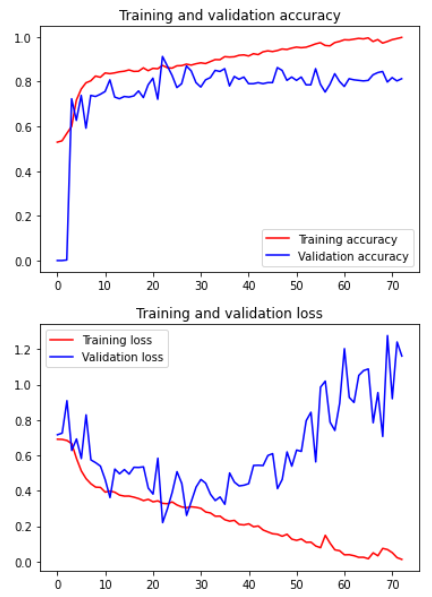
\includegraphics[width=.9\textwidth]{images/scratch_accuracy}
		\caption{Accuracy and loss graphs for the first model training}
		\label{fig:scratch_accuracy}
	\end{minipage}
	\hspace{5mm}%
	\begin{minipage}[c]{.35\textwidth}
		\centering\setlength{\captionmargin}{0pt}%
		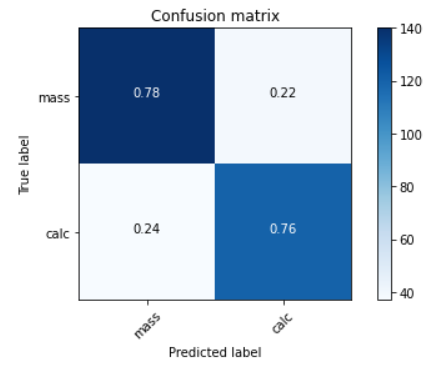
\includegraphics[width=.9\textwidth]{images/scratch_matrix}
		\caption{Confusion matrix for the test-set predictions}
		\label{fig:scratch_matrix}
	\end{minipage}%
\end{figure}

\clearpage
\subsubsection{Data augmentation}
To overcome the problem of over-fitting, we augmented our training using the \textit{ImageDataGenerator} class of \textit{keras}. The main variations we adopted were random rotation up to 40 degrees, random vertical and horizontal shifts with a range of 0.2, random zoom with a range of 0.2, random shear with a range of 0.2 and nearest fill model. To set these parameters we referred to the data in the papers we studied in the initial phase of the project. Before applying these variations to the train set, we splitted it to get the validation set separately using a validation size of the $15\%$.

\begin{figure}[h]
\centering
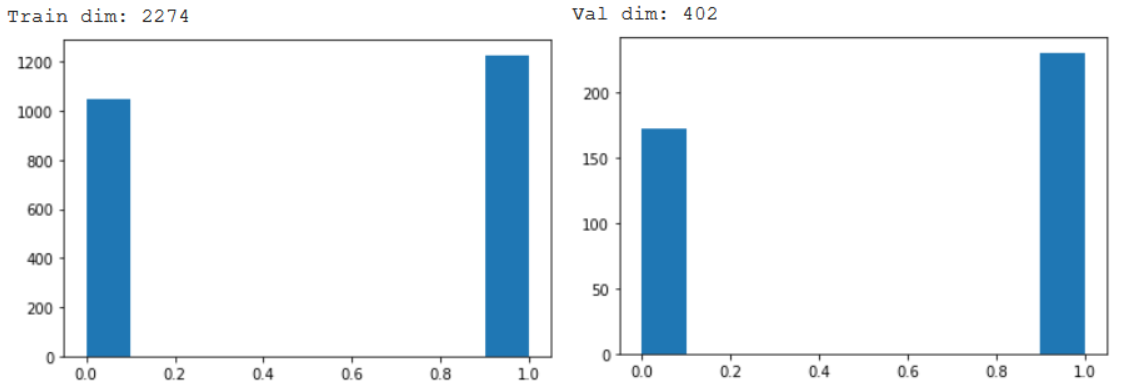
\includegraphics[width=.7\textwidth]{images/val_label_distribution}
\caption{Label distribution of the validation \\set and the training set, after the split}
\label{fig:val_label}
\end{figure}

We trained again our model with the augmented training set and with the validation set, and the results were more satisfying, having a mean accuracy over $80\%$. At this point, we wanted to have a more accurate analysis on some hyperparameters so we did several tests changing their values to get a model as good as possible. 
The tests were regarding the value of the \textit{batch size}, the number of \textit{hidden units}, the \textit{learning rate} and the \textit{optimizer} itself: we tried using the Adam optimizer and the RMSprop optimizer. Moreover, we also tested the model with different \textit{output functions}: the softmax and the sigmoid. 
The final accuracy we managed to achieve was $87\%$. This result has been obtained with the   Adam optimizer with a learning rate of $0.001$ and with the $softmax$ as the output function for the last FC layer. Regarding to the number of hidden units of the first FC layer, the differences in terms of performance were limited (1 or 2 percentage points) therefore we have chosen the smaller value ($64$), so to have a model as simple as possible. The batch size was chosen at $50$: we noticed that the $25$ batch size models returned more unstable and variable results. The architecture of the trained network is the same as in figure~\ref{fig:scratch_model}, while the results in terms of accuracy and confusion matrix of the test set are shown in figures~\ref{fig:scratch_accuracy_da} and~\ref{fig:scratch_matrix_da}.
All the tests were done with a maximum of $100$ epochs, using the early stopping with a patience of $50$.

\begin{table}[h]
\centering
\begin{tabular}{|cc|cccc|}
\hline
Batch size & Hidden units & Test accuracy & Test loss & AUC & F-score \\
\hline
25 & 64 & 0.87 & 0.30 & 0.87 & 0.86 \\ 
50 & 64 & 0.86 & 0.32 & 0.85 & 0.86 \\ 
25 & 128 & 0.80 & 0.46 & 0.80 & 0.78 \\ 
50 & 128 & 0.84 & 0.33 & 0.83 & 0.83 \\ 
25 & 256 & 0.85 & 0.33 & 0.84 & 0.83 \\ 
50 & 256 & 0.86 & 0.29 & 0.86 & 0.85 \\ 
25 & 512 & 0.88 & 0.29 & 0.88 & 0.87 \\ 
50 & 512 & 0.87 & 0.30 & 0.87 & 0.85 \\
\hline
\end{tabular}
\caption{Results of tests with Adam optimizer and softmax output function ($Task\ 2.1$)}
\end{table}

Before saving the model, we performed a $4$-holdout validation analysis to make sure that the performance remained similar to the values obtained in the previous test. 
This analysis confirmed the goodness of the model: the results of the $4$-holdout validation are shown below.

\clearpage

\begin{figure}[ht]
\centering
	\begin{minipage}[c]{.4\textwidth}
		\centering\setlength{\captionmargin}{0pt}%
		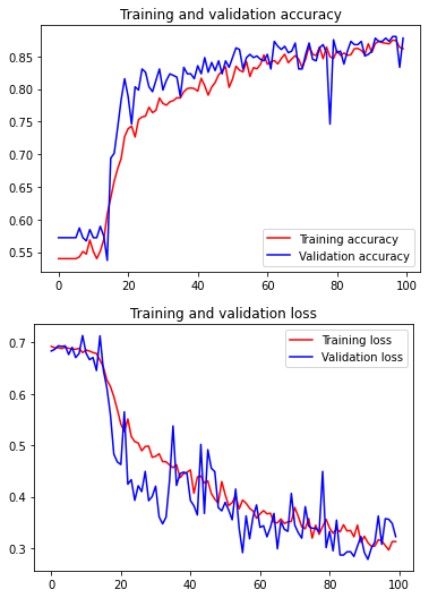
\includegraphics[width=.9\textwidth]{images/2.1-da/da_accuracy}
		\caption{Accuracy and loss graphs for the model with data augmentation}
		\label{fig:scratch_accuracy_da}
	\end{minipage}
	\hspace{5mm}%
	\begin{minipage}[c]{.4\textwidth}
		\centering\setlength{\captionmargin}{0pt}%
		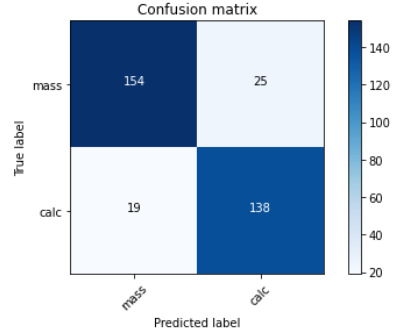
\includegraphics[width=.9\textwidth]{images/2.1-da/da_matrix}
		\caption{Confusion matrix for the test-set predictions}
		\label{fig:scratch_matrix_da}
	\end{minipage}%
\end{figure}

\begin{table}[h]
\centering
\begin{tabular}{|cccccccc|}
\hline
Batch size & Hidden units & Measure & 1st & 2nd & 3rd & 4th & \textbf{AVG} \\
\hline
\textbf{50} & \textbf{64} & accuracy & 0.87 & 0.87 & 0.85 & 0.85 & \textbf{0.86} \\
" & " & loss & 0.30 & 0.30 & 0.30 & 0.32 & \textbf{0.31} \\
" & " & AUC & 0.87 & 0.87 & 0.85 & 0.85 & \textbf{0.86} \\
" & " & F-score & 0.86 & 0.86 & 0.84 & 0.83 & \textbf{0.85} \\
\hline
\end{tabular}
\caption{Results of 4-holdout validation ($Task\ 2.1$)}
\end{table}



\subsection{Task 2.2: Benign-Malignant discriminator}
This classification was more complex to accomplish, and the results obtained are not comparable with previous experiments. One of the problems was that the distribution of the two classes was imbalanced in the training set. But the main problem was that distinguishing an abnormality patch between malignant and benign is generally more complex than distinguishing the type of abnormality. 
We spoke with a radiologist and some of his colleagues, and they explained to us that a calcification is very different to a mass: the first is always a very small abnormality, while the second one is almost always bigger. Moreover, they said that mammograms are considered first level examinations, which therefore can leave many doubts about the diagnosis. This is because there are many factors that can limit the visibility and the study of the abnormalities. 
In most cases, abnormalities are best investigated with subsequent examinations, such as ultrasound, MRI, and biopsy.
This complexity remains even in deep learning techniques.\\


As a first approach, we started from the network built in the previous task and we added some modifications, based also on the feedback found on the papers.
We used again the data augmentation, but modifying some of the parameters: in more than one paper it was specified that, to avoid too many distortions in the images, it was necessary to specify a rotation angle multiple of the right angle, and a fill mode of type 'reflect'. Moreover we disabled the horizontal flip of the image, to avoid too much differences from the original set.
We inserted a dropout layer between the two dense layers at the top of the model, with a rate varying from $0.2$ to $0.5$ in the tests.
The better results that we obtained are shown in figures~\ref{fig:accuracy_2.2} and~\ref{fig:matrix_2.2}: the used batch size was $50$, the hidden units of the first dense layer were $256$, and the optimizer was \textit{Adam} with a learning rate of $0.001$. This model was built with a rate of the dropout layer of $0.2$.

\begin{figure}[h]
\centering
	\begin{minipage}[c]{.4\textwidth}
		\centering\setlength{\captionmargin}{0pt}%
		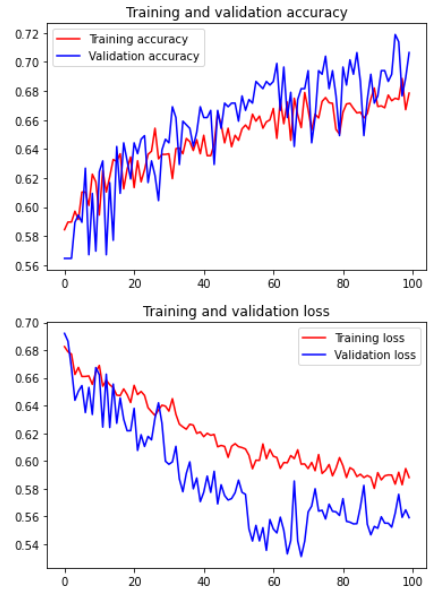
\includegraphics[width=.9\textwidth]{images/2.2/0_acc}
		\caption{Accuracy and loss graphs for the first $Task\ 2.2$ model}
		\label{fig:accuracy_2.2}
	\end{minipage}
	\hspace{5mm}%
	\begin{minipage}[c]{.4\textwidth}
		\centering\setlength{\captionmargin}{0pt}%
		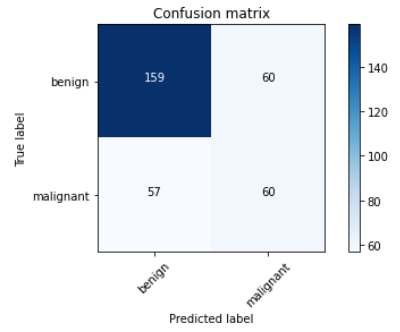
\includegraphics[width=.9\textwidth]{images/2.2/0_matrix}
		\caption{Confusion matrix for the test-set predictions}
		\label{fig:matrix_2.2}
	\end{minipage}%
\end{figure}

As we can see from the graphs, there are some improvement during the training of the network, but they're very limited and slow. We tried to increment the number of training epochs and the model started to overfitting badly. The major problem is that, predicting the test-set labels, the classifier tended to assign samples to the benign class, when we would have preferred more attention to the malignant class instead, since it is the most critical.\\

We tried to change the architecture of the model again, looking for a structure that could better capture the features of our dataset. After few attempts, we arrived at the model described in figure~\ref{fig:model_2.2_1}, in which we inserted an extra convolutional layer with $128$ kernels. We maintained the number of hidden units of the FC layer to $64$. This last choice has been made also to simplify the network, decreasing the number of parameters to train in order to reduce the overfitting. The dropout layer remained with a rate of $0.2$.

\begin{figure}[h]
\centering
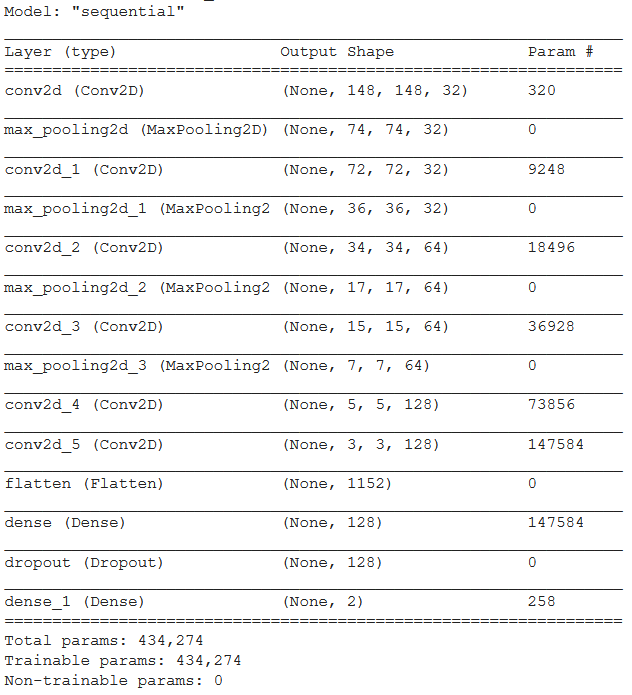
\includegraphics[width=.5\textwidth]{images/2.2/1_model}
\caption{Final architecture of the CNN from scratch ($Task\ 2.2$)}
\label{fig:model_2.2_1}
\end{figure}

\clearpage

\begin{figure}[h]
\centering
	\begin{minipage}[c]{.4\textwidth}
		\centering\setlength{\captionmargin}{0pt}%
		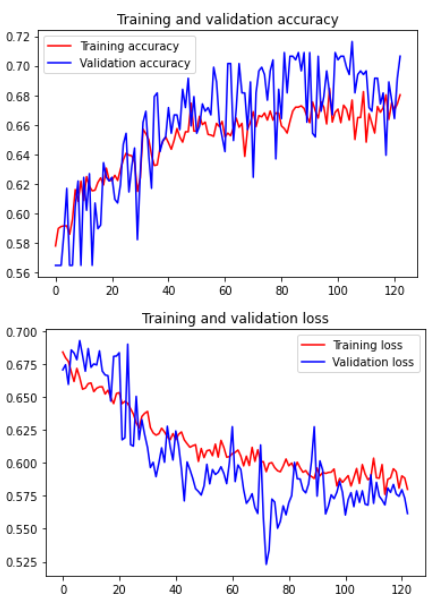
\includegraphics[width=.9\textwidth]{images/2.2/5_acc}
		\caption{Accuracy and loss graphs for the $Task\ 2.2$ model with additional convolutional layer}
		\label{fig:accuracy_2.2_1}
	\end{minipage}
	\hspace{5mm}%
	\begin{minipage}[c]{.4\textwidth}
		\centering\setlength{\captionmargin}{0pt}%
		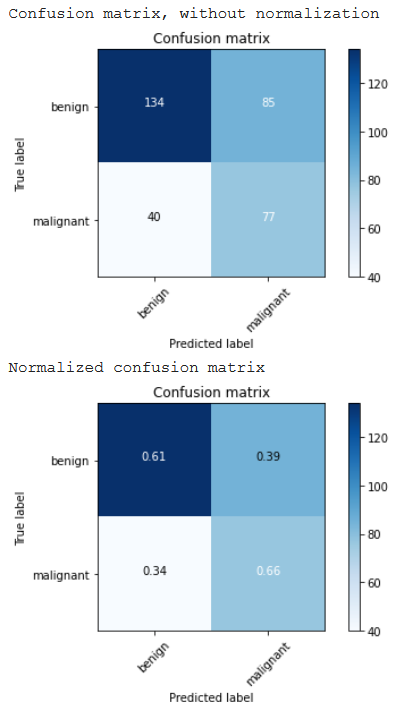
\includegraphics[width=.9\textwidth]{images/2.2/5_matrix}
		\caption{Confusion matrix for the test-set predictions}
		\label{fig:matrix_2.2_1}
	\end{minipage}%
\end{figure}

\begin{table}[h]
\centering
\begin{tabular}{|cccccccc|}
\hline
Batch size & Hidden units & Measure & 1st & 2nd & 3rd & 4th & \textbf{Avg} \\
\hline
\textbf{50} & \textbf{64} & accuracy & 0.64 & 0.66 & 0.67 & 0.65 & \textbf{0.66} \\
" & " & loss & 0.64 & 0.61 & 0.60 & 0.63 & \textbf{0.62} \\
" & " & AUC & 0.64 & 0.63 & 0.64 & 0.64 & \textbf{0.64} \\
" & " & F-score & 0.56 & 0.53 & 0.53 & 0.54 & \textbf{0.54} \\
\hline
\end{tabular}
\caption{Results of 4-holdout validation ($Task\ 2.2$)}
\label{tab:task2.2}
\end{table}

The results (fig.~\ref{fig:accuracy_2.2_1} and~\ref{fig:matrix_2.2_1}) in terms of accuracy and loss were very similar to the previous model, but we can see from the confusion matrix that the \textit{malignant} class was better predicted and we considered it as a good result.
As we can see from the table, the main problem is the value of the \textit{F-score}, that indicates a very unbalanced classification.\\

Trying to solve the unbalancing of the two classes, we assigned weights to them so that their unbalance in the training set would be considered. We have trained again the network, passing the new weights of the classes as parameters: the results are found in the figures~\ref{fig:accuracy_2.2_1_weights} and~\ref{fig:matrix_2.2_1_weights}. 

\begin{verbatim}
    weight_for_benign = (1 / benign)*(total)/2.0 
    weight_for_malignant = (1 / malignant)*(total)/2.0
    
    > Total samples: 2274
    > Benign samples: 1341
    > Malignant samples: 933
    > Weight for benign: 0.85
    > Weight for malignant: 1.22
\end{verbatim}

\clearpage

We can see that using the class weights the classifier managed to find a slightly higher number of malignant samples, at the expense of benign samples. Comparing the holdout validation tables (~\ref{tab:task2.2} and~\ref{tab:task2.2_weight}) we can see that accuracy and loss worsened, while the AUC remained almost unchanged, and the F-score increased by two percentage points. 
We also tried to change the values of the weights to see if you could improve performance further: our idea was to give even more weight to the malignant class, that was considered the most critical. But this approach did not satisfy us, because the network started to give too much importance to the class with the highest weight, and even most benign samples were classified as malignant. \\

So our choice for the final model was the version without the balanced class weights: although the F-score was higher in the one with the class weights, it paid with too much decrease of accuracy and too much increase of loss.

\begin{figure}[h]
\centering
	\begin{minipage}[c]{.4\textwidth}
		\centering\setlength{\captionmargin}{0pt}%
		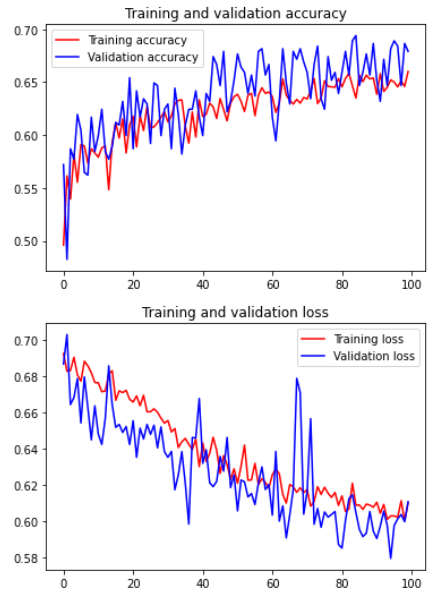
\includegraphics[width=.9\textwidth]{images/2.2/7_acc}
		\caption{Accuracy and loss graphs for the $Task\ 2.2$ model with balanced class weights}
		\label{fig:accuracy_2.2_1_weights}
	\end{minipage}
	\hspace{5mm}%
	\begin{minipage}[c]{.4\textwidth}
		\centering\setlength{\captionmargin}{0pt}%
		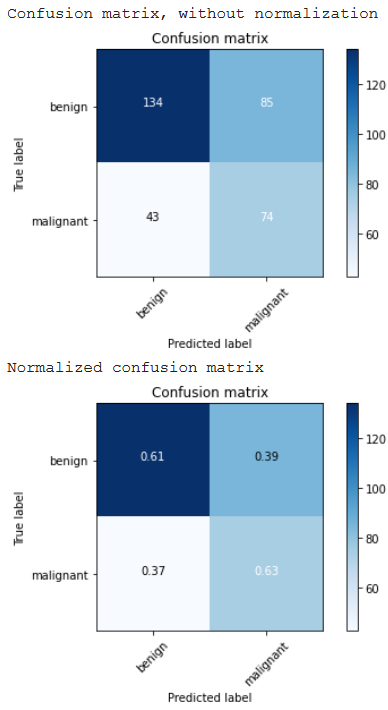
\includegraphics[width=.9\textwidth]{images/2.2/7_matrix}
		\caption{Confusion matrix for the test-set predictions}
		\label{fig:matrix_2.2_1_weights}
	\end{minipage}%
\end{figure}

\begin{table}[h]
\centering
\begin{tabular}{|cccccccc|}
\hline
Batch size & Hidden units & Measure & 1st & 2nd & 3rd & 4th & \textbf{Avg} \\
\hline
\textbf{50} & \textbf{64} & accuracy & 0.59 & 0.54 & 0.61 & 0.62 & \textbf{0.59} \\
" & " & loss & 0.66 & 0.71 & 0.64 & 0.62 & \textbf{0.66} \\
" & " & AUC & 0.64 & 0.61 & 0.64 & 0.62 & \textbf{0.63} \\
" & " & F-score & 0.57 & 0.56 & 0.57 & 0.54 & \textbf{0.56} \\
\hline
\end{tabular}
\caption{Results of 4-holdout validation with the class weights ($Task\ 2.2$)}
\label{tab:task2.2_weight}
\end{table}


\clearpage

\section{Task 3: Pretrained network}
For this task, we were inspired by some papers of works on the same dataset. Indeed, in most of the papers, pretrained networks were used to solve the classification. 
We found a study on the most used networks in the literature (shown in fig.~\ref{fig:pretrained_networks}) and then chose accordingly. The pretrained networks we worked on were:
\begin{itemize}
\item VGG-16
\item VGG-19
\item ResNet-50
\end{itemize}

\begin{figure}[h]
\centering
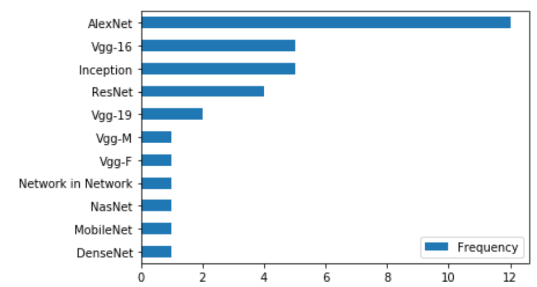
\includegraphics[width=.5\textwidth]{images/pretrained_networks}
\caption{Pretrained networks most used in the literature}
\label{fig:pretrained_networks}
\end{figure}

We used two strategies to leverage a pre-trained network. In the first one, called Feature Extraction, we started from a network trained on the “imagenet” dataset and removed the top layers and trained a new classifier on top of the output.
The second one, called Fine Tuning is similar. The main difference was that the last layer of the model base used for feature extraction was unfrozen and we trained both the newly added part of the model and these top layers. \\
The results obtained with \textit{Resnet-50} were not reported in this paper, because they weren't significant.

\subsection{Task 3.1: Mass-Calcification discriminator}
In all our tests we applied Data Augmentation because we ran into an overfitting problem.
We built a new larger training set, starting from the original images and adding two more variations for each image. Thanks to this approach, we obtained improved results, in particular overtraining has been significantly reduced. The batch size value range that achieved higher performance is between $32$ and $64$. Lower values led to high oscillations of both the training and validation loss/accuracy. For the learning rate, after testing values from 1e-4 to 1e-6, we ended up using the value of 1e-5. After testing different activation functions we ended up using “sigmoid” for the output. 

\begin{figure}[h]
\centering
	\begin{minipage}[c]{.45\textwidth}
		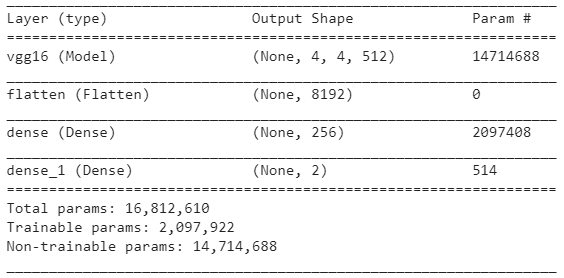
\includegraphics[width=.9\textwidth]{images/Task 3/VGG16 3.1/Model}
		\caption{Architecture of the CNN based on VGG16 ($Task\ 3.1$)}
		\label{fig:vgg16_model}
	\end{minipage}	
	\hspace{5mm}%
	\begin{minipage}[c]{.45\textwidth}
		\centering\setlength{\captionmargin}{0pt}%
		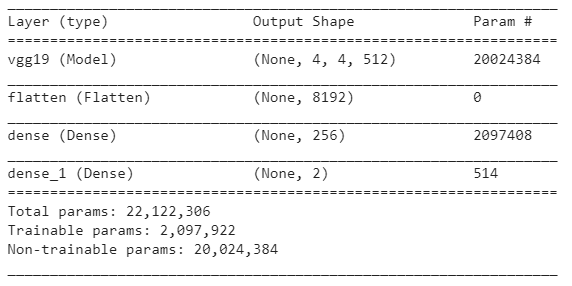
\includegraphics[width=.9\textwidth]{images/Task 3/VGG19 3.1/Model}
		\caption{Architecture of the CNN based on VGG19 ($Task\ 3.1$)}
		\label{fig:vgg19_model}
	\end{minipage}
\end{figure}

\subsubsection{Feature Extraction}
We have reported the final architecture built from the \textbf{VGG16} base in figure~\ref{fig:vgg16_model}. 
The best results were obtained with the following parameters: batch size 32, learning rate 1e-5. \\
Also from the \textbf{VGG19} convolutional base, whose architecture can be found in figure~\ref{fig:vgg19_model}, we achieved the best results with a batch size of 32 and a learning rate of 1e-5. \\
The significant results achieved are summarized in the figures~\ref{fig:vgg16_3.1_matrix_fe} and~\ref{fig:vgg19_3.1_matrix_fe}, and in the table~\ref{tab:task3.1_fe}.

\begin{figure}[h]
\centering
	\begin{minipage}[c]{.4\textwidth}
		\centering\setlength{\captionmargin}{0pt}%
		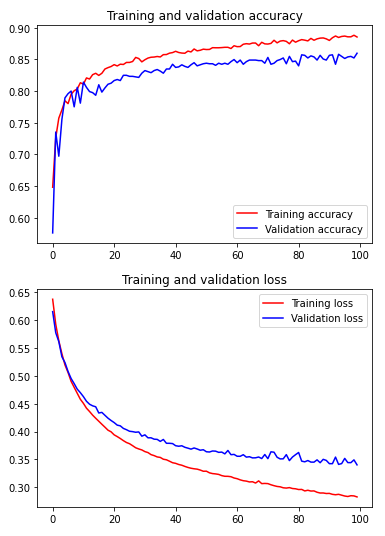
\includegraphics[width=.9\textwidth]{images/Task 3/VGG16 3.1/FE/Accuracy}
	\end{minipage}	
	\hspace{5mm}%
	\begin{minipage}[c]{.4\textwidth}
		\centering\setlength{\captionmargin}{0pt}%
		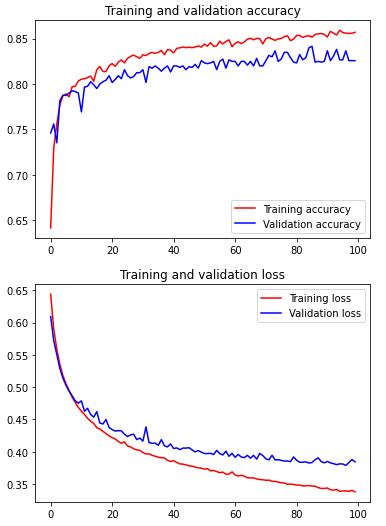
\includegraphics[width=.9\textwidth]{images/Task 3/VGG19 3.1/FE/Accuracy}
	\end{minipage}
	
	\begin{minipage}[c]{.4\textwidth}
		\centering\setlength{\captionmargin}{0pt}%
		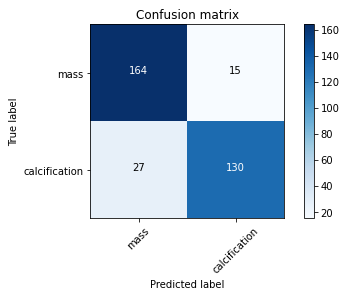
\includegraphics[width=.9\textwidth]{images/Task 3/VGG16 3.1/FE/Conf_Matrix}
		\caption{Performance for the model based on VGG16, with feature extraction}
		\label{fig:vgg16_3.1_matrix_fe}
	\end{minipage}
	\hspace{5mm}%
	\begin{minipage}[c]{.4\textwidth}
		\centering\setlength{\captionmargin}{0pt}%
		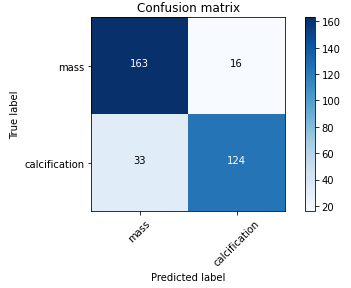
\includegraphics[width=.9\textwidth]{images/Task 3/VGG19 3.1/FE/Conf_Matrix}
		\caption{Performance for the model based on VGG19, with feature extraction}
		\label{fig:vgg19_3.1_matrix_fe}
	\end{minipage}
\end{figure}

\begin{table}[h]
\centering
\begin{tabular}{|cc|cccc|}
\hline
Model & Batch size & Test Acc & Test Loss & AUC & F-score \\
\hline
\textbf{VGG16} & 32 & \textbf{0.88} & \textbf{0.33} & \textbf{0.87} & \textbf{0.86} \\
" 	  & 64 & 0.86 & 0.34 & 0.86 & 0.85 \\
VGG19 & 32 & 0.85 & 0.37 & 0.85 & 0.83  \\
" 	  & 64 & 0.84 & 0.37 & 0.84 & 0.83 \\
\hline
\end{tabular}
\caption{Results of Feature Extraction ($Task\ 3.1$)}
\label{tab:task3.1_fe}
\end{table}

%%%%%%%%%%%%%%%%%%%%%%%%%%%%%%%%%%%%%%%%%%%%%%%%%%%%%%%%%%%%%%%%%%%%%%%%%%%%%%%%%%%%%%%%%

\clearpage

\subsubsection{Fine Tuning}
We also ran tests using the fine-tuning approach to see if we could increase classification performance.

As for VGG16, we started from the architecture in figure~\ref{fig:vgg16_model} and we carried out two different runs: the first unfreezing the pretrained network from the 5th block, while in the second the network is unfreezed from the 4th block. The results we obtained in these two cases were very similar, leading us to think that between the two would be better the first model, since it had less parameters to train. \\
Since the network tended to overtrain, we tried adding a dropout level between the two FC levels, with a rate of $0.5$. The resulting outputs showed a decrease in overtraining, as we can observe in figures~\ref{fig:vgg16_3.1_matrix_ft} and~\ref{fig:vgg16_3.1_matrix_ft_d}. 

\begin{figure}[h]
\centering
	\begin{minipage}[c]{.4\textwidth}
		\centering\setlength{\captionmargin}{0pt}%
		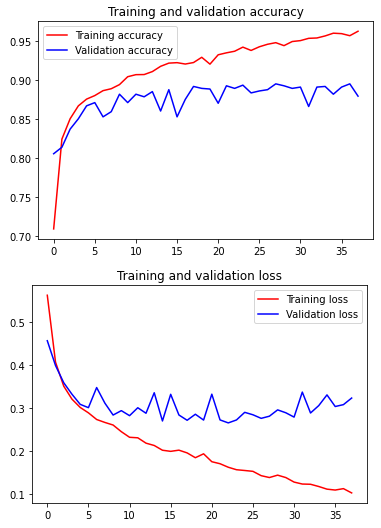
\includegraphics[width=.9\textwidth]{images/Task 3/VGG16 3.1/FT/Accuracy}
	\end{minipage}	
	\hspace{5mm}%
	\begin{minipage}[c]{.4\textwidth}
		\centering\setlength{\captionmargin}{0pt}%
		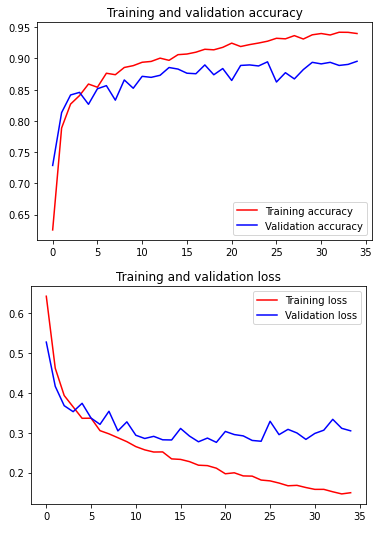
\includegraphics[width=.9\textwidth]{images/Task 3/VGG16 3.1/FT/Accuracy_drop}
	\end{minipage}
	
	\begin{minipage}[c]{.4\textwidth}
		\centering\setlength{\captionmargin}{0pt}%
		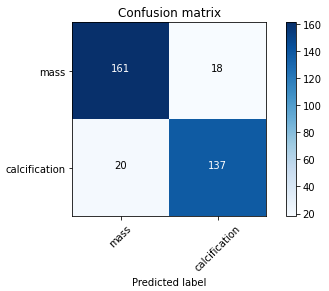
\includegraphics[width=.9\textwidth]{images/Task 3/VGG16 3.1/FT/Conf_Matrix}
		\caption{Performance for the model based on VGG16, with fine tuning}
		\label{fig:vgg16_3.1_matrix_ft}
	\end{minipage}
	\hspace{5mm}%
	\begin{minipage}[c]{.4\textwidth}
		\centering\setlength{\captionmargin}{0pt}%
		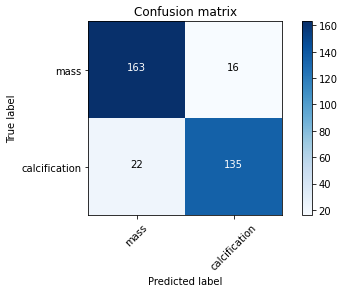
\includegraphics[width=.9\textwidth]{images/Task 3/VGG16 3.1/FT/Conf_Matrix_drop}
		\caption{Performance for the model based on VGG16, with FT and dropout}
		\label{fig:vgg16_3.1_matrix_ft_d}
	\end{minipage}
\end{figure}

Finally we re-trained VGG19, unfreezed from the 5th block: again performance was good, both with and without the dropout level. We reported a summary of all the obtained performances in the table~\ref{tab:task3.1_ft}. \\

For the final model, we saved the architecture based on VGG16, unfreezed from block 5, with the dropout level.

\clearpage

\begin{table}[h]
\centering
\begin{tabular}{|ccc|cccc|}
\hline
Model & Unfreezed block & Dropout & Test Acc & Test Loss & AUC & F-score \\
\hline
VGG16 & 5 & -   & 0.89 & 0.34 & 0.89 & 0.88 \\
\textbf{VGG16} & \textbf{5} & \textbf{0.5} & \textbf{0.89} & \textbf{0.33} & \textbf{0.89} & \textbf{0.88} \\
VGG16 & 4 & -   & 0.88 & 0.32 & 0.88 & 0.88 \\
VGG16 & 4 & 0.5 & 0.89 & 0.31 & 0.89 & 0.88 \\
VGG19 & 5 & -   & 0.85 & 0.36 & 0.85 & 0.84 \\
VGG19 & 5 & 0.5 & 0.85 & 0.36 & 0.85 & 0.84 \\
\hline
\end{tabular}
\caption{Results of Fine Tuning ($Task\ 3.1$)}
\label{tab:task3.1_ft}
\end{table}

%%%%%%%%%%%%%%%%%%%%%%%%%%%%%%%%%%%%%%%%%%%%%%%%%%%%%%%%%%%%%%%%%%%%%%%%%%%%%%%%%%%%%%%%%

\subsection{Task 3.2: Benign-Malignant discriminator}
Regarding the classification of benign and malignant abnormalities, we used the same parameters but initially the classifier failed to properly classify malignant samples. To overcome this issue we decided to modify the weight for each class: at first we set the class weights to balance the dataset, but this wasn't improving the performance of the network. So we decided to set them heuristically giving more importance to the malignant class. 

\subsubsection{Feature Extraction}
Using the \textbf{VGG16} convolutional base, the best results were obtained with the following parameters: batch size 64, learning rate 1e-5. We trained the model for 100 epochs, using an Early Stop callback with a patience of 10. These same parameters were also used for the tests with the \textbf{VGG19} base, and then for the tests with the class weights. The results are summarized in the table~\ref{tab:task3.2_fe}. \\
Using both the VGG16 and VGG19 models, we set the weight for the benign class at $1.0$, while the one for the malignant class was set to $1.25$.

\begin{table}[h]
\centering
\begin{tabular}{|cc|cccc|}
\hline
Model & Weights & Test Acc & Test Loss & AUC & F-score \\
\hline
VGG16 & -		   & 0.66 & 0.59 & 0.63 & 0.52 \\
\textbf{VGG16} & \textbf{[1.0,1.25]} & \textbf{0.69} & \textbf{0.58} & \textbf{0.64} & \textbf{0.52} \\
VGG19 & - 		   & 0.67 & 0.61 & 0.62 & 0.48 \\
VGG19 & [1.0,1.25] & 0.67 & 0.61 & 0.62 & 0.48 \\
\hline
\end{tabular}
\caption{Results of Feature Extraction ($Task\ 3.2$)}
\label{tab:task3.2_fe}
\end{table}


\subsubsection{Fine Tuning}
Since the obtained results were not very good, we decided to also try the fine tuning approach. \\
Again, we ran several tests: initially we found an overtraining problem, and for this reason, we tried to insert a dropout level before the final dense level. The dropout rate was set to $0.5$. The performance improved a bit. The table~\ref{tab:task3.2_ft} shows the most significant test results. \\

\begin{table}[h]
\centering
\begin{tabular}{|cccc|cccc|}
\hline
Model & Unfreezed block & Dropout & Weights & Test Acc & Test Loss & AUC & F-score \\
\hline
VGG16 & 5 & 0.5 & [1.0,1.25] & 0.66 & 0.60 & 0.61 & 0.47 \\
VGG16 & 5 & 0.5 & - 	     & 0.68 & 0.60 & 0.61 & 0.47 \\
\textbf{VGG19} & \textbf{5} & \textbf{0.5} & \textbf{[1.0,1.25]} & \textbf{0.65} & \textbf{0.62} & \textbf{0.63} & \textbf{0.53} \\
VGG19 & 5 & 0.5 & -	   	     & 0.66 & 0.62 & 0.63 & 0.52 \\
\hline
\end{tabular}
\caption{Results of Fine Tuning ($Task\ 3.2$)}
\label{tab:task3.2_ft}
\end{table}

\clearpage

As we can observe from the previous summary tables, with regard to the technique of feature extraction the model that has resulted better is the one based on VGG16 with the class weights, while for the fine tuning the best one is based on VGG19, again with the class weights. The graphs of accuracy and loss trends, together with the confusion matrices of these two models, are found in the figures~\ref{fig:vgg16_3.2} and~\ref{fig:vgg19_3.2}. Between the two, as final model, we chose the VGG16-based, because in addition to have better performance it presented less overfitting.


\begin{figure}[h]
\centering
	\begin{minipage}[c]{.4\textwidth}
		\centering\setlength{\captionmargin}{0pt}%
		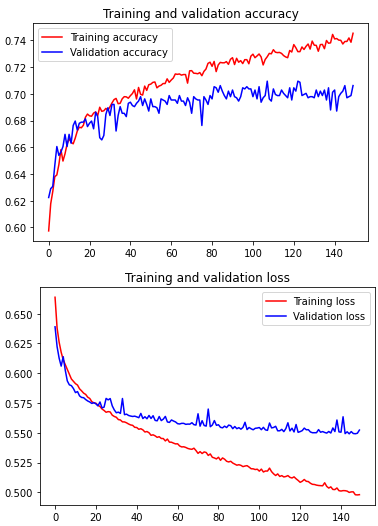
\includegraphics[width=.9\textwidth]{images/Task 3/VGG16 3.2/Accuracy}
	\end{minipage}	
	\hspace{5mm}%
	\begin{minipage}[c]{.4\textwidth}
		\centering\setlength{\captionmargin}{0pt}%
		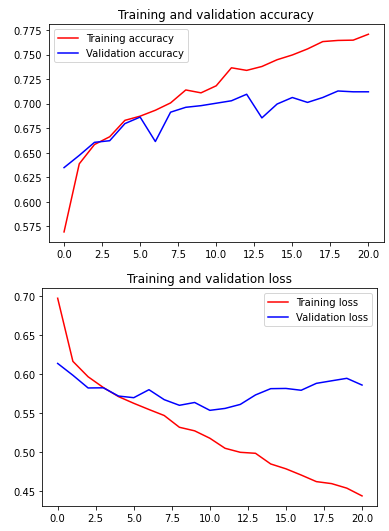
\includegraphics[width=.9\textwidth]{images/Task 3/VGG19 3.2/Accuracy}
	\end{minipage}
	
	\begin{minipage}[c]{.4\textwidth}
		\centering\setlength{\captionmargin}{0pt}%
		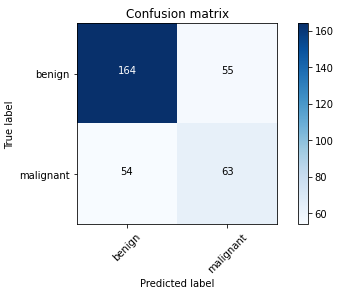
\includegraphics[width=.9\textwidth]{images/Task 3/VGG16 3.2/Conf_Matrix}
		\caption{Performance for the \textbf{VGG16} based model, with FE and class weights}
		\label{fig:vgg16_3.2}
	\end{minipage}
	\hspace{5mm}%
	\begin{minipage}[c]{.4\textwidth}
		\centering\setlength{\captionmargin}{0pt}%
		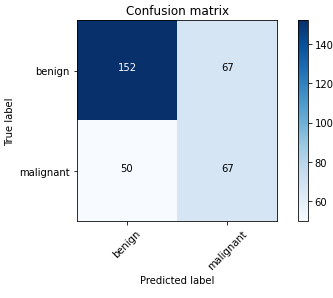
\includegraphics[width=.9\textwidth]{images/Task 3/VGG19 3.2/Conf_Matrix}
		\caption{Performance for the \textbf{VGG19} based model, with FT and class weights}
		\label{fig:vgg19_3.2}
	\end{minipage}
\end{figure}

\clearpage

\section{Task 4: Baseline patches}
For this part of the project, we planned to integrate the baseline patches, the ones extracted from healthy tissues in the mammograms, into the classifiers identified so far. Our goal was to test whether adding the baseline patch samples into the training set would help the model better identify and learn features related to the abnormalities.
We focused on the classification between mass and calcification. \\
So we started from the model architecture built from scratch in the $Task\ 2.1$ (fig.~\ref{fig:scratch_model}), and changed the number of output units to $3$. We carried out some tests, modifying the hyper-parameters, to see the effect that the baseline patches had on the network training.

We initially trained with the architecture as it was, using again a batch size of $50$, the softmax as output function, and the Adam optimizer with the default learning rate. Moreover we have maintained the use of data augmentation. The obtained results are found in figures~\ref{fig:4_acc} and~\ref{fig:4_matrix}. We can see that the performance are good, around the $80\%$ of accuracy and F-score, but not as good as the model witouth the baseline. 

\begin{figure}[h]
\centering
	\begin{minipage}[c]{.4\textwidth}
		\centering\setlength{\captionmargin}{0pt}%
		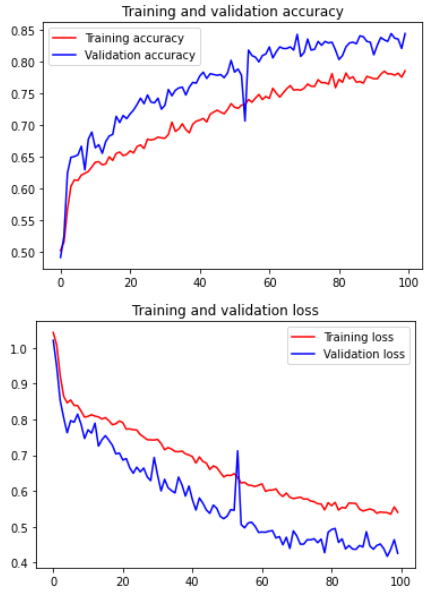
\includegraphics[width=.9\textwidth]{images/4.1/1_acc}
		\caption{Accuracy and loss graphs for the model based on the CNN from scratch ($Task\ 4$)}
		\label{fig:4_acc}
	\end{minipage}
	\hspace{5mm}%
	\begin{minipage}[c]{.4\textwidth}
		\centering\setlength{\captionmargin}{0pt}%
		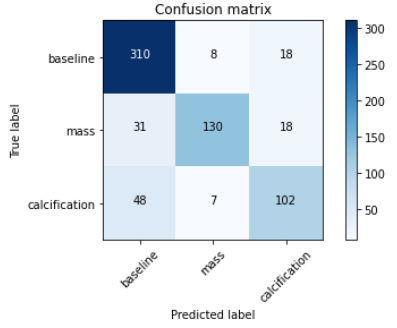
\includegraphics[width=.9\textwidth]{images/4.1/1_matrix}
		\caption{Confusion matrix for the test-set predictions}
		\label{fig:4_matrix}
	\end{minipage}%
\end{figure}

We thought this was due to the large imbalance in the dataset: in fact, the number of baseline patch samples was twice as large as the number of masses/calcifications. We therefore performed a subsequent test by rebalancing the class weights:
\begin{verbatim}
    weight_for_baseline = (1 / baseline)*(total)/3.0 
    weight_for_mass = (1 / mass)*(total)/3.0
    weight_for_calcification = (1 / calcification)*(total)/3.0
    
    > Tot. samples: 4549
    > Bas. samples: 2282, weight: 0.66
    > Mass samples: 1041, weight: 1.46
    > Calc samples: 1226, weight: 1.24
\end{verbatim}

\begin{figure}[h]
\centering
	\begin{minipage}[c]{.4\textwidth}
		\centering\setlength{\captionmargin}{0pt}%
		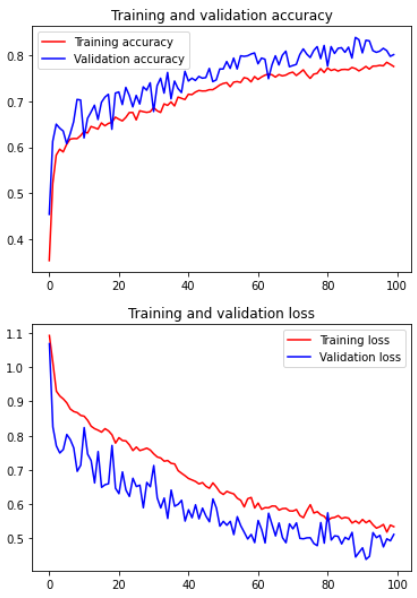
\includegraphics[width=.9\textwidth]{images/4.1/2_acc}
		\caption{Accuracy and loss graphs for the model based on the CNN from scratch ($Task\ 4$)}
		\label{fig:4_acc_w}
	\end{minipage}
	\hspace{5mm}%
	\begin{minipage}[c]{.4\textwidth}
		\centering\setlength{\captionmargin}{0pt}%
		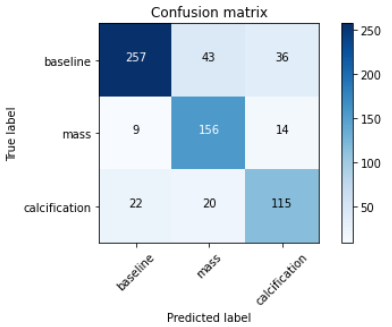
\includegraphics[width=.9\textwidth]{images/4.1/2_matrix}
		\caption{Confusion matrix for the test-set predictions}
		\label{fig:4_matrix_w}
	\end{minipage}%
\end{figure}

Here as in other tests, rebalancing the weights did not bring much improvement. However, we can see that mass and calcification classification improved, by $14\%$ and $8\%$ respectively, but at the expense of baseline classification which worsened by $16\%$. What we noticed in general, even in other tests that we did not report, is that calcifications are the abnormalities that are most often confused: in our opinion this is due to the fact that, as the radiologists with whom we were in contact had explained to us, calcifications are much smaller than masses, and consequently it could be more difficult to capture their features for neural networks, and confuse them with other classes.

\begin{table}
\centering
	\begin{tabular}{|cccc|}
	\hline
	Model & Test Accuracy & Test Loss & F-score \\
	\hline
	batch:50, hidden u:64 & 0.83 & 0.46 & 0.80 \\
	"    with weights & 0.79 & 0.57 & 0.79 \\
	\hline
	\end{tabular}
\caption{Summary of the performance of the $Task\ 4$ tests}
\end{table}

\subsection{Siamese Network}
Since the previous approach did not bring the expected results, we tried another approach, based on the architecture called Siamese Network. The idea was to send as input to the two identical networks of the model pairs of images, respectively to one a baseline patch and to the other an abnormality patch (mass or calcification).

At the output of the Flatten layer of the two common networks, we obtained the features extracted from the input and with a Lambda layer we performed the subtraction between the abnormality and baseline patch features. Our hope was that, from this difference, the most relevant features would be highlighted and the classification between masses and calcifications would improve. \\
The final architecture we used is shown in figure~\ref{fig:siamese_model}: we started from the convolutional base of VGG16, keeping all blocks frozen. The we did an additional test, trying to unfreeze the convolutional base from the 5th block. The results of these tests are shown in the figures~\ref{fig:siamese_fe} and~\ref{fig:siamese_ft}: note that the Early Stop callback was used with a patience of 10 and with the best weights restoring mode activated.

\begin{figure}[h]
\centering
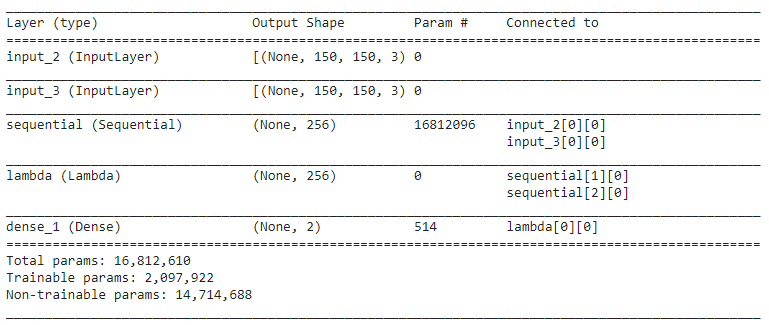
\includegraphics[width=.5\textwidth]{images/4.1/Siamese/Model}
\caption{Architecture of the Siamese Network}
\label{fig:siamese_model}
\end{figure}

\begin{figure}[h]
\centering
	\begin{minipage}[c]{.35\textwidth}
		\centering\setlength{\captionmargin}{0pt}%
		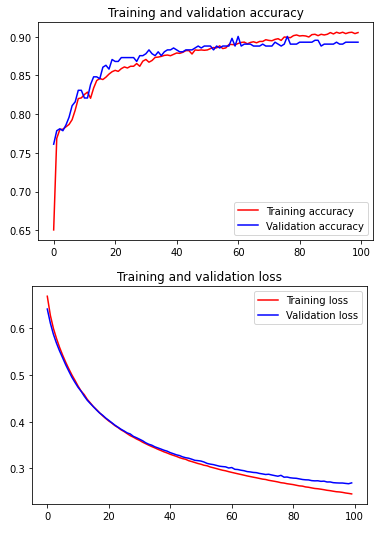
\includegraphics[width=.9\textwidth]{images/4.1/Siamese/Accuracy_fe}
		\caption{Accuracy and loss graphs for the Siamese Network (feature extraction)}
		\label{fig:scratch_accuracy}
	\end{minipage}
	\hspace{5mm}%
	\begin{minipage}[c]{.35\textwidth}
		\centering\setlength{\captionmargin}{0pt}%
		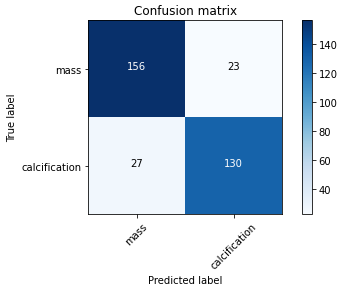
\includegraphics[width=.9\textwidth]{images/4.1/Siamese/Conf_Matrix_fe}
		\caption{Confusion matrix for the test-set predictions}
		\label{fig:scratch_matrix}
	\end{minipage}%
\end{figure}

\begin{figure}[h]
\centering
	\begin{minipage}[c]{.4\textwidth}
		\centering\setlength{\captionmargin}{0pt}%
		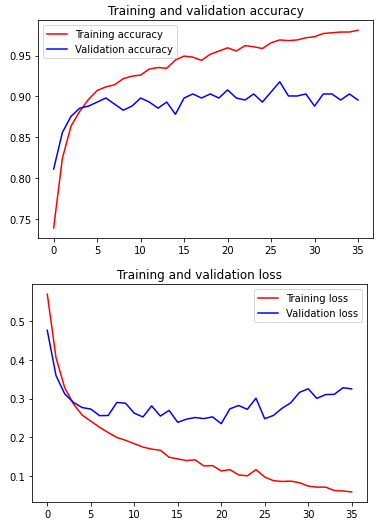
\includegraphics[width=.9\textwidth]{images/4.1/Siamese/AccuracyFT}
	\end{minipage}	
	\hspace{5mm}%
	\begin{minipage}[c]{.4\textwidth}
		\centering\setlength{\captionmargin}{0pt}%
		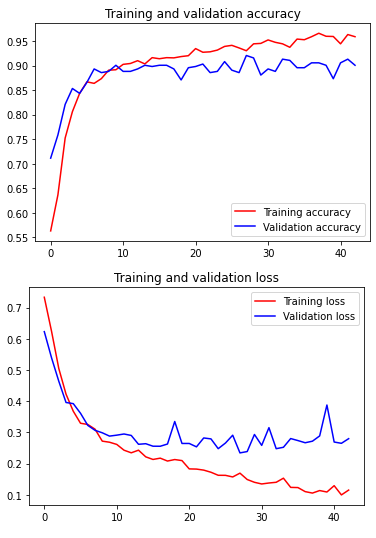
\includegraphics[width=.9\textwidth]{images/4.1/Siamese/AccuracyFT_drop}
	\end{minipage}
	
	\begin{minipage}[c]{.4\textwidth}
		\centering\setlength{\captionmargin}{0pt}%
		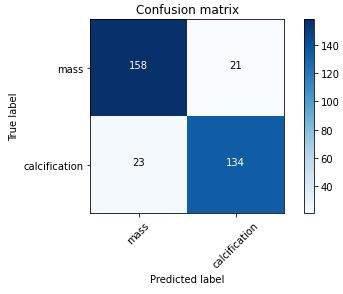
\includegraphics[width=.9\textwidth]{images/4.1/Siamese/Conf_MatrixFT}
		\caption{Performance for the Siamese Network, with FT}
		\label{fig:siamese_fe}
	\end{minipage}
	\hspace{5mm}%
	\begin{minipage}[c]{.4\textwidth}
		\centering\setlength{\captionmargin}{0pt}%
		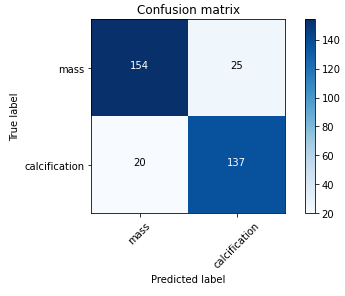
\includegraphics[width=.9\textwidth]{images/4.1/Siamese/Conf_MatrixFT_drop}
		\caption{Performance for the Siamese Network, with FT and dropout}
		\label{fig:siamese_ft}
	\end{minipage}
\end{figure}

\begin{table}
\centering
	\begin{tabular}{|ccc|cccc|}
	\hline
	Model & Unfreezed block & Dropout & Test Accuracy & Test Loss & AUC & F-score \\
	\hline
	VGG16 & - & -   & 0.86 & 0.34 & 0.86 & 0.85 \\
	"     & 5 & -   & 0.87 & 0.33 & 0.87 & 0.86 \\
	"	  & 5 & 0.5 & 0.87 & 0.34 & 0.87 & 0.86 \\
	\hline
	\end{tabular}
\caption{Summary of the performance of the Siamese Network tests}
\end{table}

\clearpage

\section{Task 5: Ensemble network}
For the last task, we took the best models saved so far and merged them into a single network with a final additional layer, averaging over the outputs. This procedure was performed for both the mass-calcification classification and the benign-malignant classification.

\subsection{Mass-Calcification discriminator}

\begin{figure}[h]
\centering
	\begin{minipage}[c]{.9\textwidth}
		\centering\setlength{\captionmargin}{0pt}%
		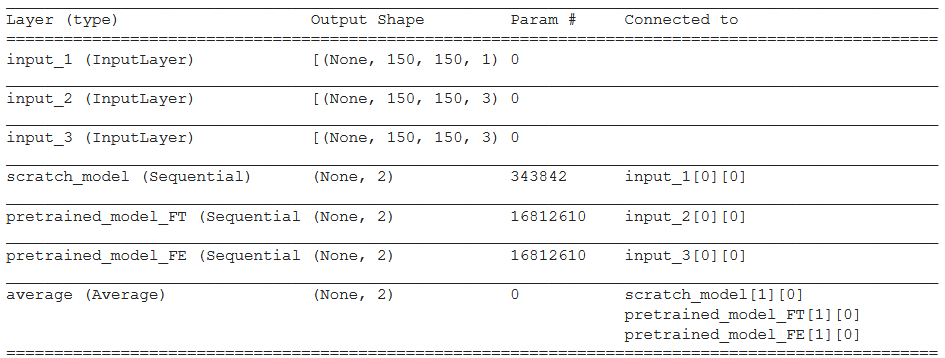
\includegraphics[width=.9\textwidth]{images/5/1_model}
		\caption{ Ensemble network for the mass-calcification classification}
	\end{minipage}
	
	\begin{minipage}[c]{.45\textwidth}
		\centering\setlength{\captionmargin}{0pt}%
		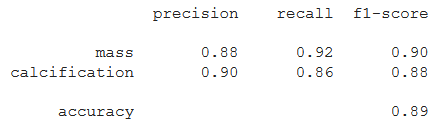
\includegraphics[width=.9\textwidth]{images/5/1_accuracy}
	\end{minipage}	
	\hspace{5mm}%
	\begin{minipage}[c]{.45\textwidth}
		\centering\setlength{\captionmargin}{0pt}%
		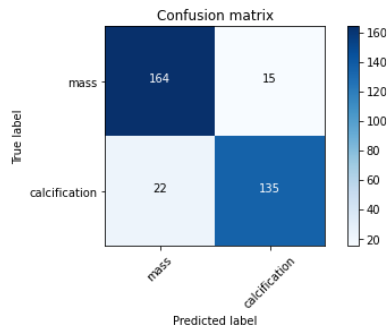
\includegraphics[width=.9\textwidth]{images/5/1_matrix}
	\end{minipage}
\end{figure}

\begin{table}[h]
\centering
	\begin{tabular}{|c|ccc|}
	\hline
	Model & Test Accuracy & AUC & F-score \\
	\hline
	scratch\_model 		  & 0.87 & 0.87 & 0.86 \\
	pretrained\_model\_FT & 0.89 & 0.89 & 0.88 \\
	pretrained\_model\_FE & 0.88 & 0.87 & 0.86 \\
	\textbf{ensemble}     & \textbf{0.89} & \textbf{0.89} & \textbf{0.88} \\
	\hline
	\end{tabular}
\caption{Single model performance vs Ensemble performance}
\end{table}

\clearpage

\subsection{Benign-Malignant discriminator}

\begin{figure}[h]
\centering
	\begin{minipage}[c]{.9\textwidth}
		\centering\setlength{\captionmargin}{0pt}%
		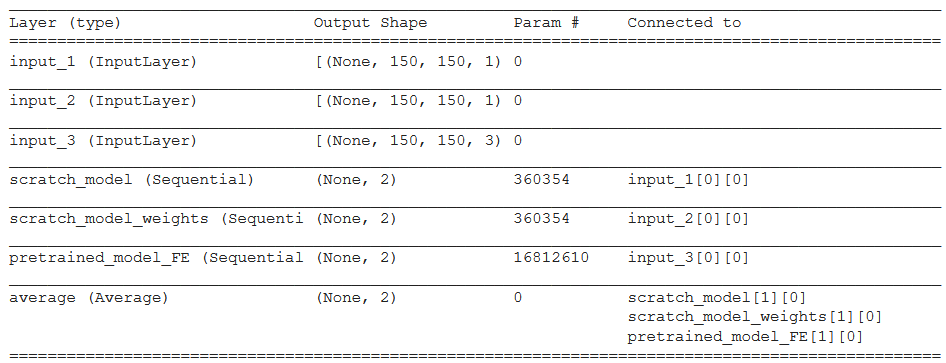
\includegraphics[width=.9\textwidth]{images/5/2_model}
		\caption{ Ensemble network for the benign-malignant classification}
	\end{minipage}
	
	\begin{minipage}[c]{.45\textwidth}
		\centering\setlength{\captionmargin}{0pt}%
		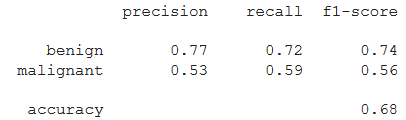
\includegraphics[width=.9\textwidth]{images/5/2_accuracy}
	\end{minipage}	
	\hspace{5mm}%
	\begin{minipage}[c]{.45\textwidth}
		\centering\setlength{\captionmargin}{0pt}%
		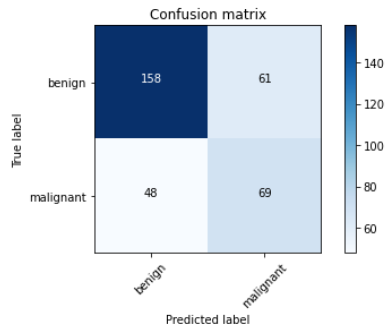
\includegraphics[width=.9\textwidth]{images/5/2_matrix}
	\end{minipage}
\end{figure}

\begin{table}[h]
\centering
	\begin{tabular}{|c|ccc|}
	\hline
	Model & Test Accuracy & AUC & F-score \\
	\hline
	scratch\_model 			& 0.65 & 0.64 & 0.54 \\
	scratch\_model\_weights & 0.62 & 0.62 & 0.54 \\
	pretrained\_model\_FE   & 0.69 & 0.64 & 0.52 \\
	\textbf{ensemble} 		& \textbf{0.68} & \textbf{0.66} & \textbf{0.56} \\
	\hline
	\end{tabular}
\caption{Single model performance vs Ensemble performance}
\end{table}

\end{document}
